\documentclass[border=10pt]{standalone}

\usepackage{tikz}
\usepackage{tikzsymbols}
\usetikzlibrary{calc,patterns,shapes.geometric}

\def\centerarc[#1](#2)(#3:#4:#5){\draw[#1] ($(#2)+({#5*cos(#3)},{#5*sin(#3)})$) arc (#3:#4:#5);}

\begin{document}
	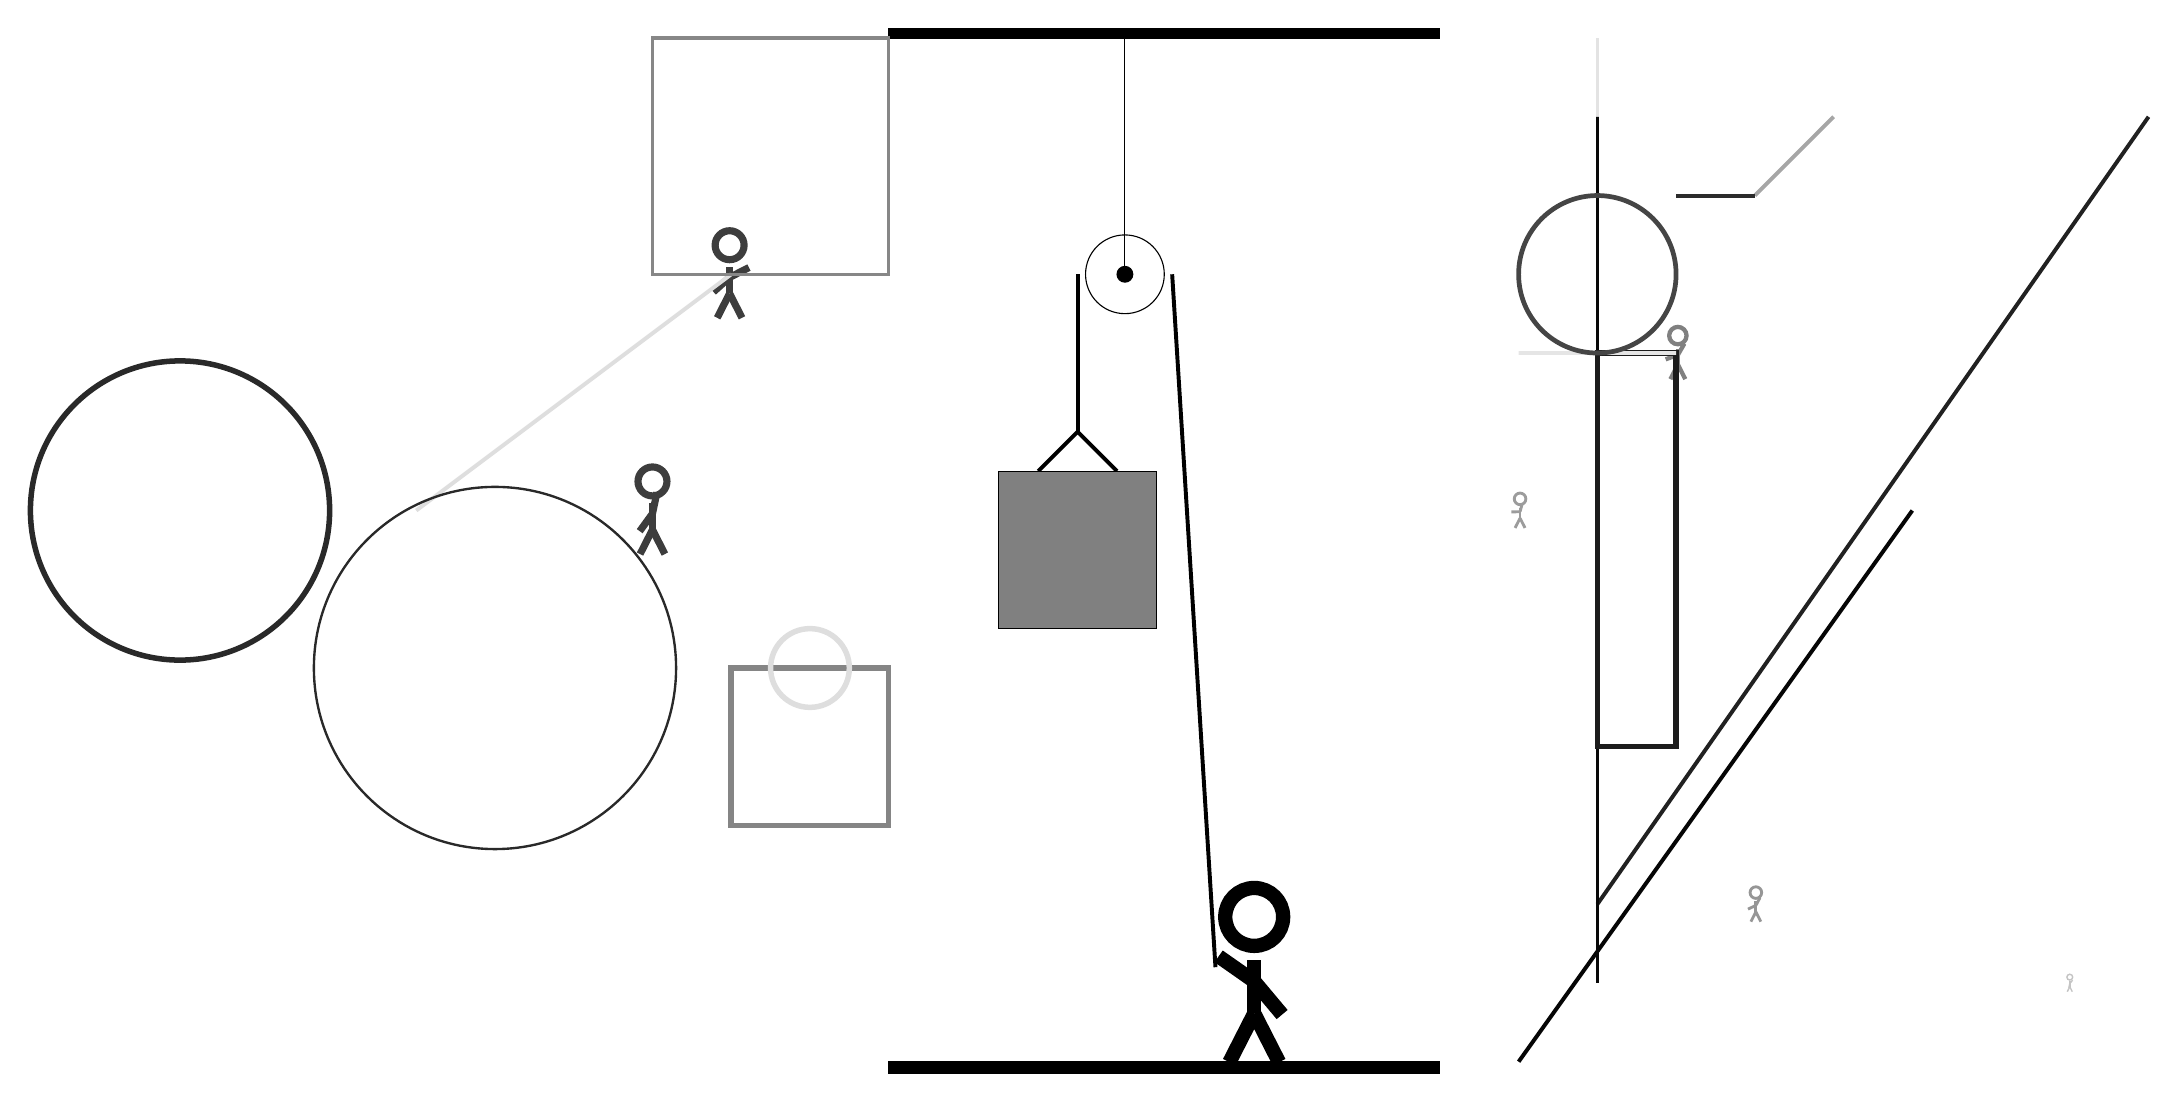
\begin{tikzpicture}
		%%%%% START %%%%%
		
		\draw[fill=black] (-2, 10) rectangle (5, 10.125);
		
		\draw (1, 7) circle (0.5);
		\draw[fill=black] (1, 7) circle (0.1);
		\draw (1, 10) -- (1, 7);
		
		\draw[line width=0.5mm] (-0.1, 4.5) -- (0.4, 5.0) -- (0.9, 4.5);
		\draw[fill=black!50] (-0.6, 4.5) rectangle (1.4, 2.5);
		
		\draw[line width=0.5mm] (0.4, 7) -- (0.4, 5.0);
		\centerarc[line width=0.5mm](1, 7)(0:180:0.6);
		\draw[line width=0.5mm](1.6, 7) -- (2.15, -1.8);
		
		\node[line width=0.7mm, color=black!76] at (-4, 7) {\Strichmaxerl[5][42][27]};
		
		\draw[line width=0.5mm, color=black!13](-4, 7) -- (-8, 4);
		\node[line width=0.4mm, color=black!41] at (9, -1) {\Strichmaxerl[2][25][62]};
		\node[line width=0.6mm, color=black!39] at (6, 4) {\Strichmaxerl[2][1][75]};
		
		\draw[line width=0.5mm, color=black!98](6, -3) -- (11, 4);
		\draw [line width=0.7mm, color=black!84](-11, 4) circle (1.9);
		\draw[line width=0.5mm, color=black!87](7, -1) -- (14, 9);
		\draw[line width=0.4mm, color=black!11] (7, 2) rectangle (7, 10);
		\draw[line width=0.7mm, color=black!48] (-4, 0) rectangle (-2, 2);
		\draw[line width=0.4mm, color=black!47] (-2, 10) rectangle (-5, 7);
		
		\node[line width=0.6mm, color=black!50] at (8, 6) {\Strichmaxerl[3][20][60]};
		
		\node[line width=0.6mm, color=black!23] at (13, -2) {\Strichmaxerl[1][77][51]};
		\draw[line width=0.5mm, color=black!35](9, 8) -- (10, 9);
		
		\draw[line width=0.4mm, color=black!97] (7, -2) rectangle (7, 9);
		\draw[line width=0.7mm, color=black!89] (7, 1) rectangle (8, 6);
		\draw[line width=0.5mm, color=black!83](8, 8) -- (9, 8);
		
		\node[line width=0.4mm, color=black!76] at (-5, 4) {\Strichmaxerl[5][54][78]};
		\draw[line width=0.4mm, color=black!10] (6, 6) rectangle (8, 6);
		\draw [line width=0.7mm, color=black!13](-3, 2) circle (0.5);
		\draw [line width=0.3mm, color=black!84](-7, 2) circle (2.3);
		\draw [line width=0.6mm, color=black!73](7, 7) circle (1.0);
		
		
		\node at (2.6, -1.9) {\Strichmaxerl[10][-35][-50]};
		
		\draw[fill=black] (-2, -3) rectangle (5, -3.15);
		
		%%%%% END %%%%%
	\end{tikzpicture}
\end{document}